% Copyright 2021 Fausto Spoto
%
% Licensed under the Apache License, Version 2.0 (the "License");
% you may not use this file except in compliance with the License.
% You may obtain a copy of the License at
%
%    http://www.apache.org/licenses/LICENSE-2.0
%
% Unless required by applicable law or agreed to in writing, software
% distributed under the License is distributed on an "AS IS" BASIS,
% WITHOUT WARRANTIES OR CONDITIONS OF ANY KIND, either express or implied.
% See the License for the specific language governing permissions and
% limitations under the License.

\documentclass[11pt]{beamer}  %% versione proiettore
%%\documentclass[11pt,handout]{beamer} %% versione stampa
\usepackage{lucidiJb-2ed}
\usepackage{mathtools}
\usepackage{relsize}
\usepackage[normalem]{ulem}

\mode<article>
{
  \usepackage{fullpage}
  \usepackage{hyperref}
}

\mode<presentation>
{
  \setbeamertemplate{background canvas}[vertical shading][bottom=red!10,top=blue!10]
  \usetheme{Course}
  \usefonttheme[onlysmall]{structurebold}
}

\subtitle{Blockchain Course}
\title{Hotmoka}
\institute{Universit\`a di Verona, Italy}
\date{March 2021}

\setbeamercovered{invisible}

\def\codesize{\smaller}
\def\<#1>{\codeid{#1}}
\newcommand{\codeid}[1]{\ifmmode{\mbox{\codesize\ttfamily{#1}}}\else{\codesize\ttfamily #1}\fi}

\begin{document}

\begin{frame}
  \titlepage
\end{frame}

\begin{frame}
  \frametitle{Hotmoka}

  \begin{greenbox}{\url{https://github.com/Hotmoka/hotmoka}}
    An open-source implementation of a network of nodes:
    \begin{itemize}
    \item nodes of a blockchain
    \item IoT devices
    \item computers in the cloud
    \end{itemize}
  \end{greenbox}

  \bigskip

  \begin{greenbox}{Requests are OO-based}
    \begin{itemize}
    \item create an object
    \item call a method of an object
    \item methods are implemented in a subset of Java
    \end{itemize}
  \end{greenbox}

\end{frame}

\begin{frame}\frametitle{Documentation}

  \begin{greenbox}{}
    There is an online tutorial on Hotmoka and Takamaka:

    \url{https://github.com/Hotmoka/hotmoka}
  \end{greenbox}

  \bigskip

  \begin{greenbox}{}
    Its many examples of Takamaka projects are available here:

    \url{https://github.com/Hotmoka/hotmoka_tutorial}
  \end{greenbox}

\end{frame}

\begin{frame}\frametitle{The API of a Hotmoka node}

  \begin{itemize}
  \item \<[add|post]JarStore(request):TransactionReference>
  \item \<[add|post]ConstructorCall(request):StorageReference>
  \item \<[add|post|run]InstanceMethodCall(request):StorageValue>
  \item \<[add|post|run]StaticMethodCall(request):StorageValue>
  \item \<subscribeToEvents(key):Subscription>
  \item \<getState(StorageReference):State>
  \end{itemize}

  \bigskip

  \begin{greenbox}{}
    \<add> calls are synchronous (wait for the result)

    \smallskip
    \<post> calls are asynchronous (yield a future)

    \smallskip
    \<run> calls are synchronous and only for read-only methods
  \end{greenbox}

\end{frame}

\begin{frame}\frametitle{Nodes can be Tendermint applications}

  \begin{center}
    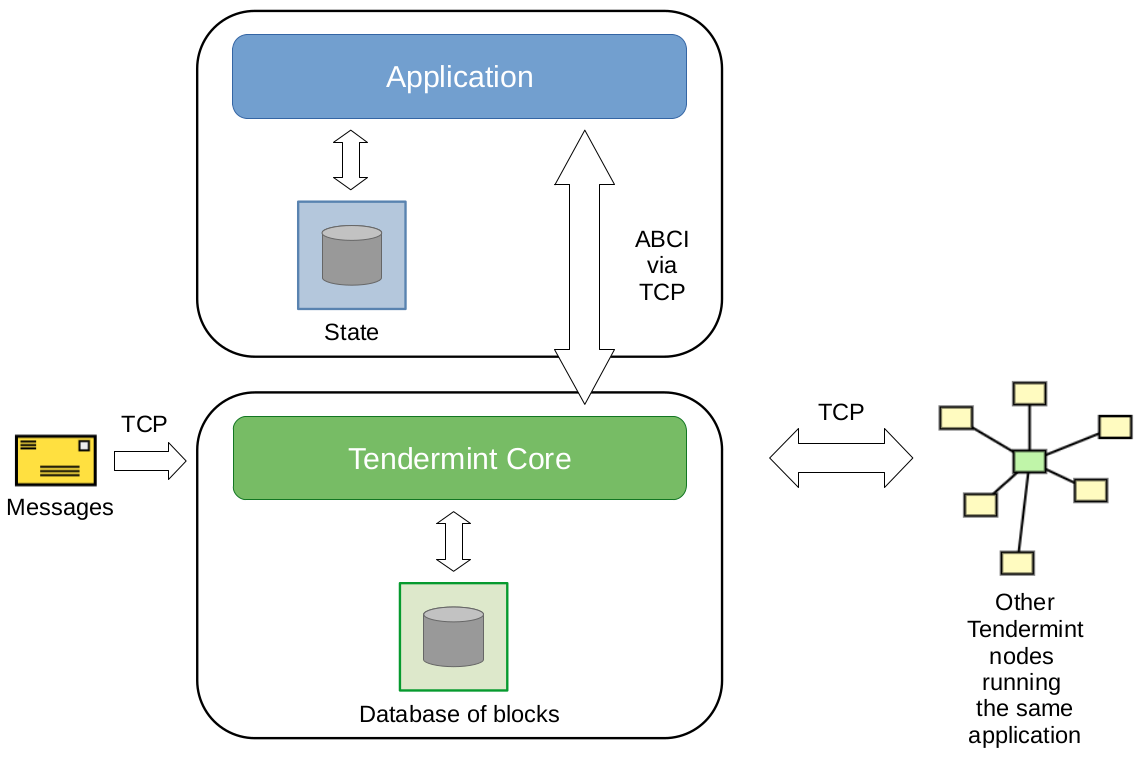
\includegraphics[width=\textwidth,clip=false]{pictures/tendermint-databases.png}
  \end{center}
    
\end{frame}

\begin{frame}\frametitle{An OO state (hash is sha256)}

  \begin{center}
    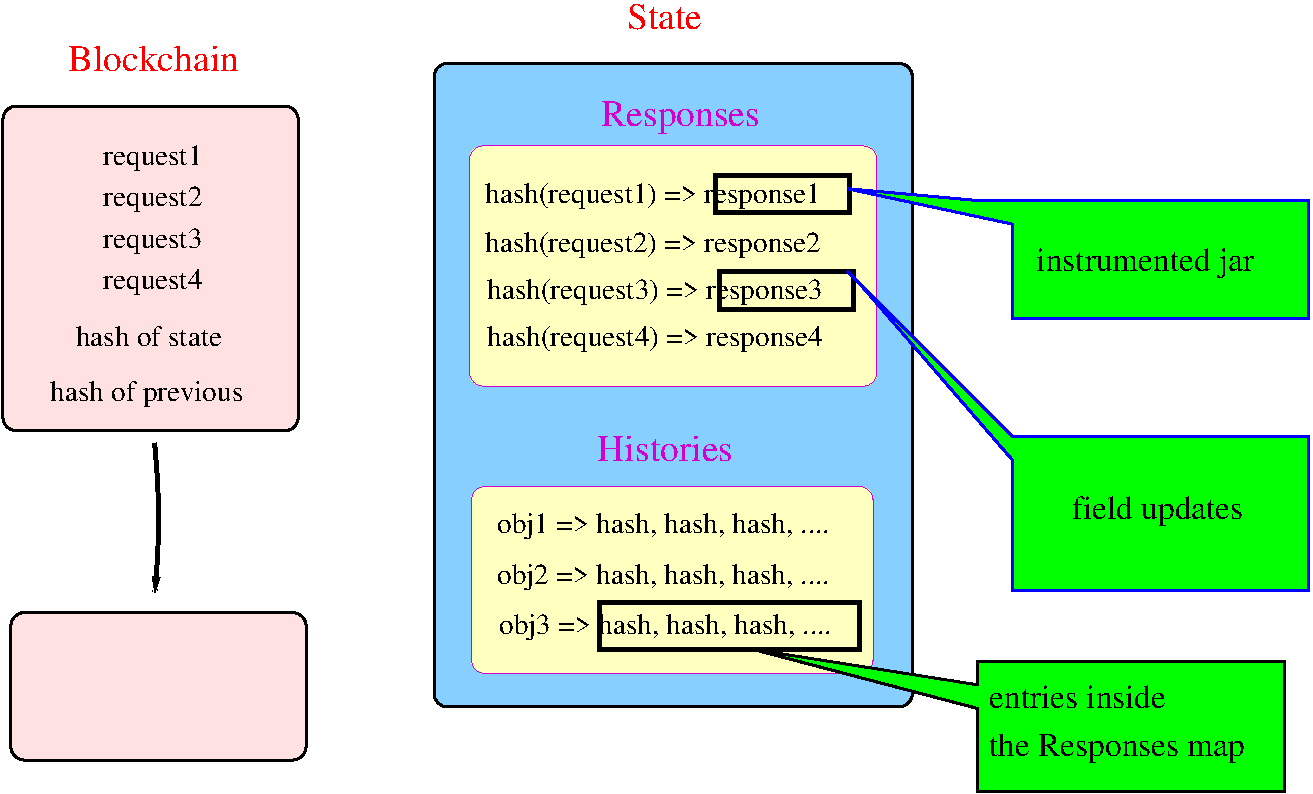
\includegraphics[width=\textwidth,clip=false]{pictures/hotmoka-structure.pdf}
  \end{center}

\end{frame}

\begin{frame}\frametitle{The API of the state}
  
    \begin{enumerate}
    \item get jar at \<hash>: access the Responses map and find the jar
    \item get object at \<obj>: access the Histories at \<obj>: for each \<hash>
      there, access the Responses map at \<hash>, project the updates on \<obj>
      and reconstruct the state of \<obj>
    \item put request/response in state: expand Responses with hash(request)$\Rightarrow$response
      \begin{itemize}
      \item[] if the response contains updates, add hash(request) to the histories of
        the updated objects
      \end{itemize}
    \item \<h=get\_hash()>: compute the hash of the hash of the Merkle-Patricia trie for
      Responses and of that for Histories
    \item \sout{\<checkout(h)>} $\Rightarrow$ unused data from points above are garbage-collected
    \end{enumerate}

\end{frame}

\begin{frame}\frametitle{The execution of a method (or constructor)}

  \begin{greenbox}{The request}
    \begin{itemize}
    \item payer object, receiver object and actual arguments (\emph{input})
    \item classpath, signature of the method
    \item nonce, chain id, gas price, gas limit
    \item signature of the request
    \end{itemize}
  \end{greenbox}

  \bigskip

  \begin{greenbox}{The computation of the response (ie, the execution of the request)}
    \begin{enumerate}
    \item find the jar(s) in state for the classpath
    \item reconstruct, from the state, RAM objects for \emph{input}
    \item execute the method on a normal Java Virtual Machine (in RAM)
    \item at the end, identify updates to fields of objects reachable from \emph{input}
      or return value
    \item pack those updates into a response (RAM objects destroyed now)
    \item put request/response in state
    \end{enumerate}
  \end{greenbox}

\end{frame}

\begin{frame}[fragile]\frametitle{How can Hotmoka identify updates to fields of objects?}

  \begin{greenbox}{The original code}
    \begin{semiverbatim}
      public class C \{
        public {\color{blue}int i;}
        public void foo() \{
          {\color{blue}i} = 42;
        \}
      \}
    \end{semiverbatim}
  \end{greenbox}

  \begin{center}
    No way to know if \<i> changed its value during the execution of \<foo()>
  \end{center}

\end{frame}

\begin{frame}[fragile]\frametitle{How can Hotmoka identify updates to fields of objects?}

  \begin{greenbox}{The instrumented code}
    \begin{semiverbatim}
      public class C {\color{red}extends Storage} \{
        public {\color{blue}int i, old\_i;} // alias at method start
        public void foo() \{
          {\color{blue}i} = 42;
        \}
      \}
    \end{semiverbatim}
  \end{greenbox}

  \begin{center}
    \<i> changed its value during the execution of \<foo()> iff at the end \<i>$\not=$\<old\_i>
  \end{center}

\end{frame}

\begin{frame}[fragile]\frametitle{How can Hotmoka enforce gas limits?}

  \begin{greenbox}{The original code}
    \begin{semiverbatim}
      public class C \{
        public void foo() \{
          while (...) \{
            ...
          \}
        \}
      \}
    \end{semiverbatim}
  \end{greenbox}

  \begin{center}
    This might loop for very long or even forever
  \end{center}

\end{frame}

\begin{frame}[fragile]\frametitle{How can Hotmoka enforce gas limits?}

  \begin{greenbox}{The instrumented code}
    \begin{semiverbatim}
      {\color{blue}static long counter;}
      public class C \{
        public void foo() \{
          while (...) \{
            {\color{blue}if (counter++ >= gaslimit)
              throw new OutOfGasError();}
            ...
          \}
        \}
      \}
    \end{semiverbatim}
  \end{greenbox}

  \begin{center}
    Actual gas costs are more fine-grained
  \end{center}

\end{frame}

\begin{frame}\frametitle{Verification and instrumentation of jars in state}

  Each jar that gets installed in a Hotmoka node undergoes two processes:

  \begin{enumerate}
  \item Verification: absence of frequent errors
    \begin{itemize}
    \item objects stored in state extend \<Storage>
    \item non-deterministic or non-terminating library code is not used
    \item no synchronization
    \item no native code
    \item no \emph{dangerous} bytecodes
    \item no finalizers
    \item no static fields (mostly)
    \item code annotations are used correctly
    \item \ldots
    \end{itemize}
  \item Instrumentation
    \begin{itemize}
    \item fields of \<Storage> classes get duplicated
    \item gas metering is weaved into the code
    \item code annotations get implemented \emph{by magic}
    \item \ldots
    \end{itemize}
  \end{enumerate}

\end{frame}

\begin{frame}\frametitle{The Takamaka programming language}

  Takamaka is the subset of Java that passes the verification
  of a Hotmoka node. It uses code annotations to implement contract-based aspects:

  \begin{itemize}
  \item {\color{blue}\<@FromContract>} annotates something that can only be called by a contract,
    not by any other code; hence, it has a {\color{blue}\<caller()>}
  \item {\color{blue}\<@Payable>} annotates something whose execution requires to pay some
    cryptocurrency units
  \item {\color{blue}\<@View>} annotates something whose execution can be run for free,
    without paying for its gas: it must not generate any update at its end
    (\emph{pure} code)
  \end{itemize}

  \bigskip
  Takamaka comes equipped with a {\color{blue}support library}
  (\<io-takamaka-code>) that defines such annotations and
  other typical classes that are useful
  for programming smart contracts

\end{frame}

\begin{frame}[fragile]\frametitle{How to program in Takamaka}

  \begin{enumerate}
  \item download Hotmoka

    {\color{blue}\<git clone git@github.com:Hotmoka/hotmoka.git>}

  \item let Maven compile and install it in your local repository

    {\color{blue}\<mvn clean install -DskipTests>}

  \item all Takamaka projects can now refer to this Maven dependency in their \<pom.xml>:
\vspace*{-3ex}\begin{semiverbatim}
{\color{blue}{
<dependency>
  <groupId>io.hotmoka</groupId>
  <artifactId>io-takamaka-code</artifactId>
  <version>1.0.0</version>
</dependency>
}}\end{semiverbatim}

  \end{enumerate}

\end{frame}

\begin{frame}[fragile]\frametitle{A first example of Takamaka code}

  \begin{enumerate}
  \item create a new Java Maven project (skip archetype selection)
  \item edit the Maven configuration file \<pom.xml> as follows:
\vspace*{-1ex}{\tiny\begin{semiverbatim}
{\color{blue}{
<project ...>
  <modelVersion>4.0.0</modelVersion>

  {\color{armygreen}<groupId>io.hotmoka</groupId>
  <artifactId>ponzi</artifactId>
  <version>0.0.1</version>}

  {\color{violet}{<properties>
    <project.build.sourceEncoding>UTF-8</project.build.sourceEncoding>
    <maven.compiler.source>11</maven.compiler.source>
    <maven.compiler.target>11</maven.compiler.target>
    <failOnMissingWebXml>false</failOnMissingWebXml>
  </properties>}}

  {\color{red}{<dependencies> <dependency>
      <groupId>io.hotmoka</groupId>
      <artifactId>io-takamaka-code</artifactId>
      <version>1.0.0</version>
  </dependency> </dependencies>}}

  {\color{violet}{<build> <plugins> <plugin>
        <groupId>org.apache.maven.plugins</groupId>
        <artifactId>maven-compiler-plugin</artifactId>
        <version>3.8.1</version>
        <configuration> <release>11</release> </configuration>
  </plugin> </plugins> </build>}}

</project>
}}\end{semiverbatim}}
  \end{enumerate}

\end{frame}

\begin{frame}[fragile]\frametitle{A first example of Takamaka code}

  \begin{enumerate}
    \setcounter{enumi}{2}
  \item create a source package \<io.takamaka.ponzi> inside \<src/main/java>
  \item create a \<module-info.java> in the \<src/main/java> directory:
    \vspace*{-3ex}\begin{semiverbatim}
{\color{blue}{
module ponzi \{
  requires io.takamaka.code;
\}
}}\end{semiverbatim}
  \end{enumerate}

\end{frame}

\begin{frame}[fragile]\frametitle{A first example of Takamaka code}

  \begin{enumerate}
    \setcounter{enumi}{4}
      \item add the following class in package \<io.takamaka.ponzi>
\vspace*{-1ex}{\tiny\begin{semiverbatim}
{\color{darkblue}{
package io.takamaka.ponzi;

import static io.takamaka.code.lang.Takamaka.require;
import java.math.BigInteger;
import io.takamaka.code.lang.Contract;
import io.takamaka.code.lang.FromContract;
import io.takamaka.code.lang.Payable;
import io.takamaka.code.lang.PayableContract;
import io.takamaka.code.lang.View;

public class SimplePonzi {\color{red}extends Contract} \{
  private final BigInteger _10 = BigInteger.valueOf(10L), _11 = BigInteger.valueOf(11L);
  private {\color{armygreen}PayableContract} currentInvestor;
  private BigInteger currentInvestment = BigInteger.ZERO;

  public {\color{violet}@Payable} {\color{armygreen}@FromContract(PayableContract.class)} void invest({\color{violet}BigInteger amount}) \{
    BigInteger minimum = currentInvestment.multiply(_11).divide(_10);
    require(amount.compareTo(minimum) >= 0, () -> "you must invest at least " + minimum);
    currentInvestor.{\color{armygreen}receive(amount)};
    currentInvestor = {\color{armygreen}(PayableContract) caller()};
    currentInvestment = amount;
  \}

  public {\color{red}@View} BigInteger getCurrentInvestment() \{
    return currentInvestment;
  \}
\}
}}\end{semiverbatim}}
  \end{enumerate}

\end{frame}

\begin{frame}[fragile]\frametitle{A first example of Takamaka code}

  \begin{enumerate}
    \setcounter{enumi}{5}
  \item compile everything with Maven:

    {\color{blue}\<mvn package>}

  \item the compiled jar of your project will appear inside the
    directory \<target> of your project, ready to be installed in a
    Hotmoka node
  \end{enumerate}
\end{frame}

\end{document}
